\section{Question 1}

\subsection{Question}
\verbatiminput{q1/q1.txt}

\subsection{Answer}
To complete this assignment, a blog word count dataset was required. To start off, a list of blog URIs was obtained using the method described in class, implemented as the {\tt get\_uris.py} script, which can be found in Appendix A, Listing \ref{listing:get_uris}. Two default blogs, F-Measure and the Old Dominion Web Science and Digital Libraries blogs, were added as defaults to the initial URI list and then, using the seed URI provided (Listing \ref{listing:default}), the remaining 98 URIs from random blogs within the blogger.com family were added.

\lstinputlisting[language=Python, caption={main for get\_uris.py}, label=listing:geturis:main, linerange={27-39}, firstnumber=27]{q1/get_uris.py}

\lstinputlisting[language=Python, caption={referenced variables in get\_uris.py}, label=listing:default, linerange={7-8}, firstnumber=7]{q1/get_uris.py}

The {\tt get\_uris main} function in Listing \ref{listing:geturis:main} was the driver that called the {\tt get\_atom} function (shown in Listing \ref{listing:geturis:atom}) to extract the atom \cite{atom} URIs from each blog and add them to the set of URIs with the {\tt add\_uri} function, shown in Listing \ref{listing:geturis:adduri}.

\clearpage

\lstinputlisting[language=Python, caption={get\_atom function}, label=listing:geturis:atom, linerange={10-19}, firstnumber=10]{q1/get_uris.py}

\lstinputlisting[language=Python, caption={add\_uri function}, label=listing:geturis:adduri, linerange={21-25}, firstnumber=21]{q1/get_uris.py}

After the full list of 100 URIs was obtained page counts for each blog were extraced and saved to a file called {\tt pagecounts} using the {\tt matrix.py} script. This script is a modified version of {\tt generatefeedvectors.py} from the book {\it Programming Collective Intelligence} \cite{pci} and can be found in full in Appendix A, Listing \ref{listing:matrix}. 

The code responsible for downloading the blogs and counting the words in each is shown in Listing \ref{listing:matrix:get}, which calls the {\tt get\_titles}, {\tt get\_words} and {\tt get\_next} functions found in Listing \ref{listing:matrix:gettitles}. This code loops over the list of URIs that was created with the {\tt get\_uris.py} script (Listing \ref{listing:get_uris}), parses each entry, and extracts all the words in each entry's title. 

\lstinputlisting[language=Python, caption={looping over the URIs}, label=listing:matrix:get, linerange={95-105}, firstnumber=95]{matrix.py}

\clearpage

\lstinputlisting[language=Python, caption={processing each blog}, label=listing:matrix:gettitles, linerange={9-38}, firstnumber=9]{matrix.py}

The parsed results were then read by the code in Listing \ref{listing:matrix:loadwrite}. This code used the {\tt load\_data} functions in Listing \ref{listing:matrix:loaddata} and \ref{listing:matrix:buildwordlist} to read each of the blog word counts and then created four collections to organize them all:

\begin{enumerate}
	\item {\tt apcount}: A dictionary containing the count for all words combined
	\item {\tt wordcounts}: A dictionary containing each blog's individual word count
	\item {\tt pagecounts}: A dictionary containing each blog's page count
	\item {\tt wordlist}: A list containing all of the words found in each blog
\end{enumerate}

\lstinputlisting[language=Python, caption={creating the blog data matrix}, label=listing:matrix:loadwrite, linerange={107-115}, firstnumber=107]{matrix.py}

\clearpage

\lstinputlisting[language=Python, caption={loading the data}, label=listing:matrix:loaddata, linerange={50-69}, firstnumber=50]{matrix.py}

\lstinputlisting[language=Python, caption={building the master wordlist}, label=listing:matrix:buildwordlist, linerange={71-77}, firstnumber=71]{matrix.py}

The code in Listing \ref{listing:matrix:writedata} then created the matrix using the {\tt write\_data} function.

\lstinputlisting[language=Python, caption={writing the data}, label=listing:matrix:writedata, linerange={79-93}, firstnumber=79]{matrix.py}

To build a histogram showing the blog page counts, the {\tt pagecounts} file was parsed by the R script in Listing \ref{listing:hist} and saved as a pdf, which is shown in Figure \ref{fig:hist}.

\lstinputlisting[language=R, caption={building the histogram}, label=listing:hist]{q1/build_histogram.r}

\clearpage

\begin{figure}[h!]
\centering
\fbox{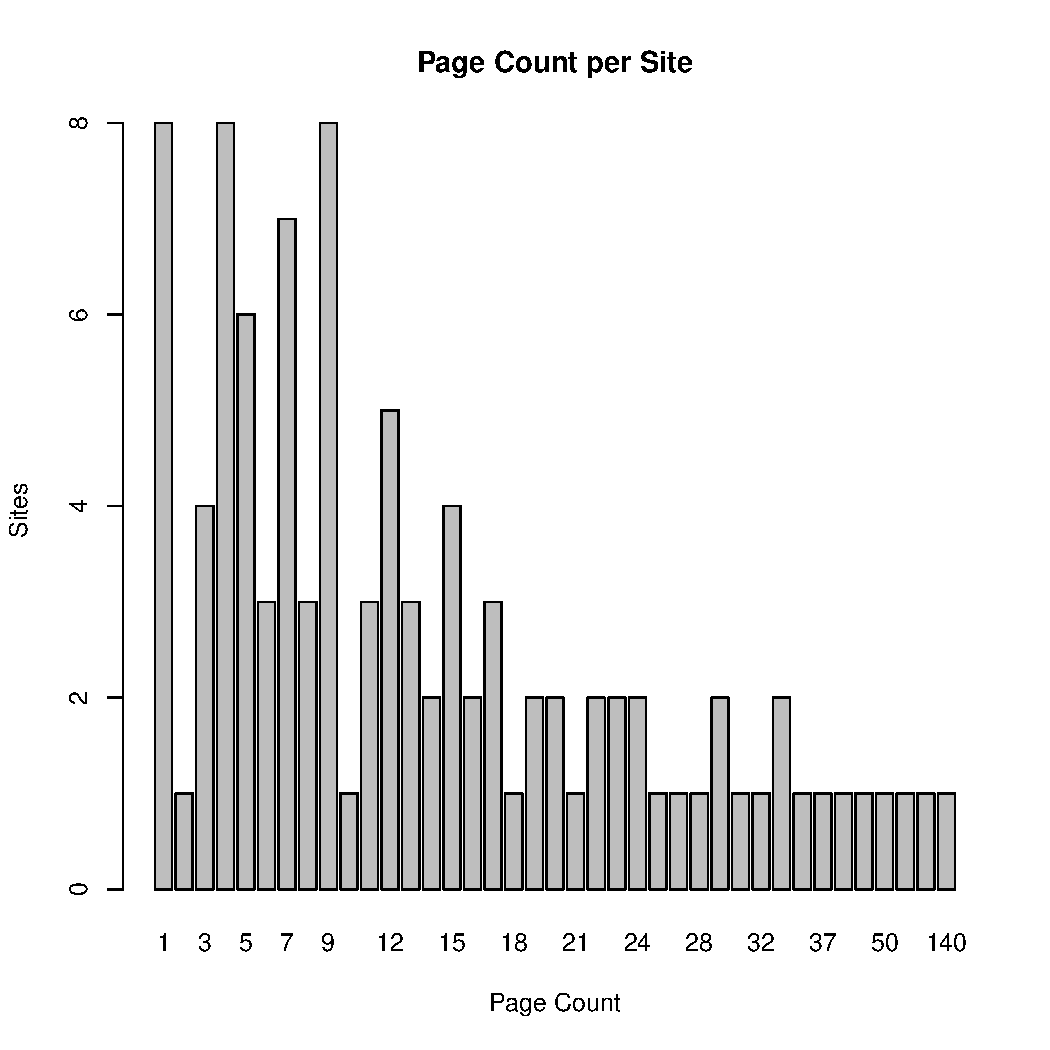
\includegraphics[scale=0.75]{q1/hist.pdf}}
\caption{Page Count per Blog}
\label{fig:hist}
\end{figure}